\begin{figure*}[t]
\centering
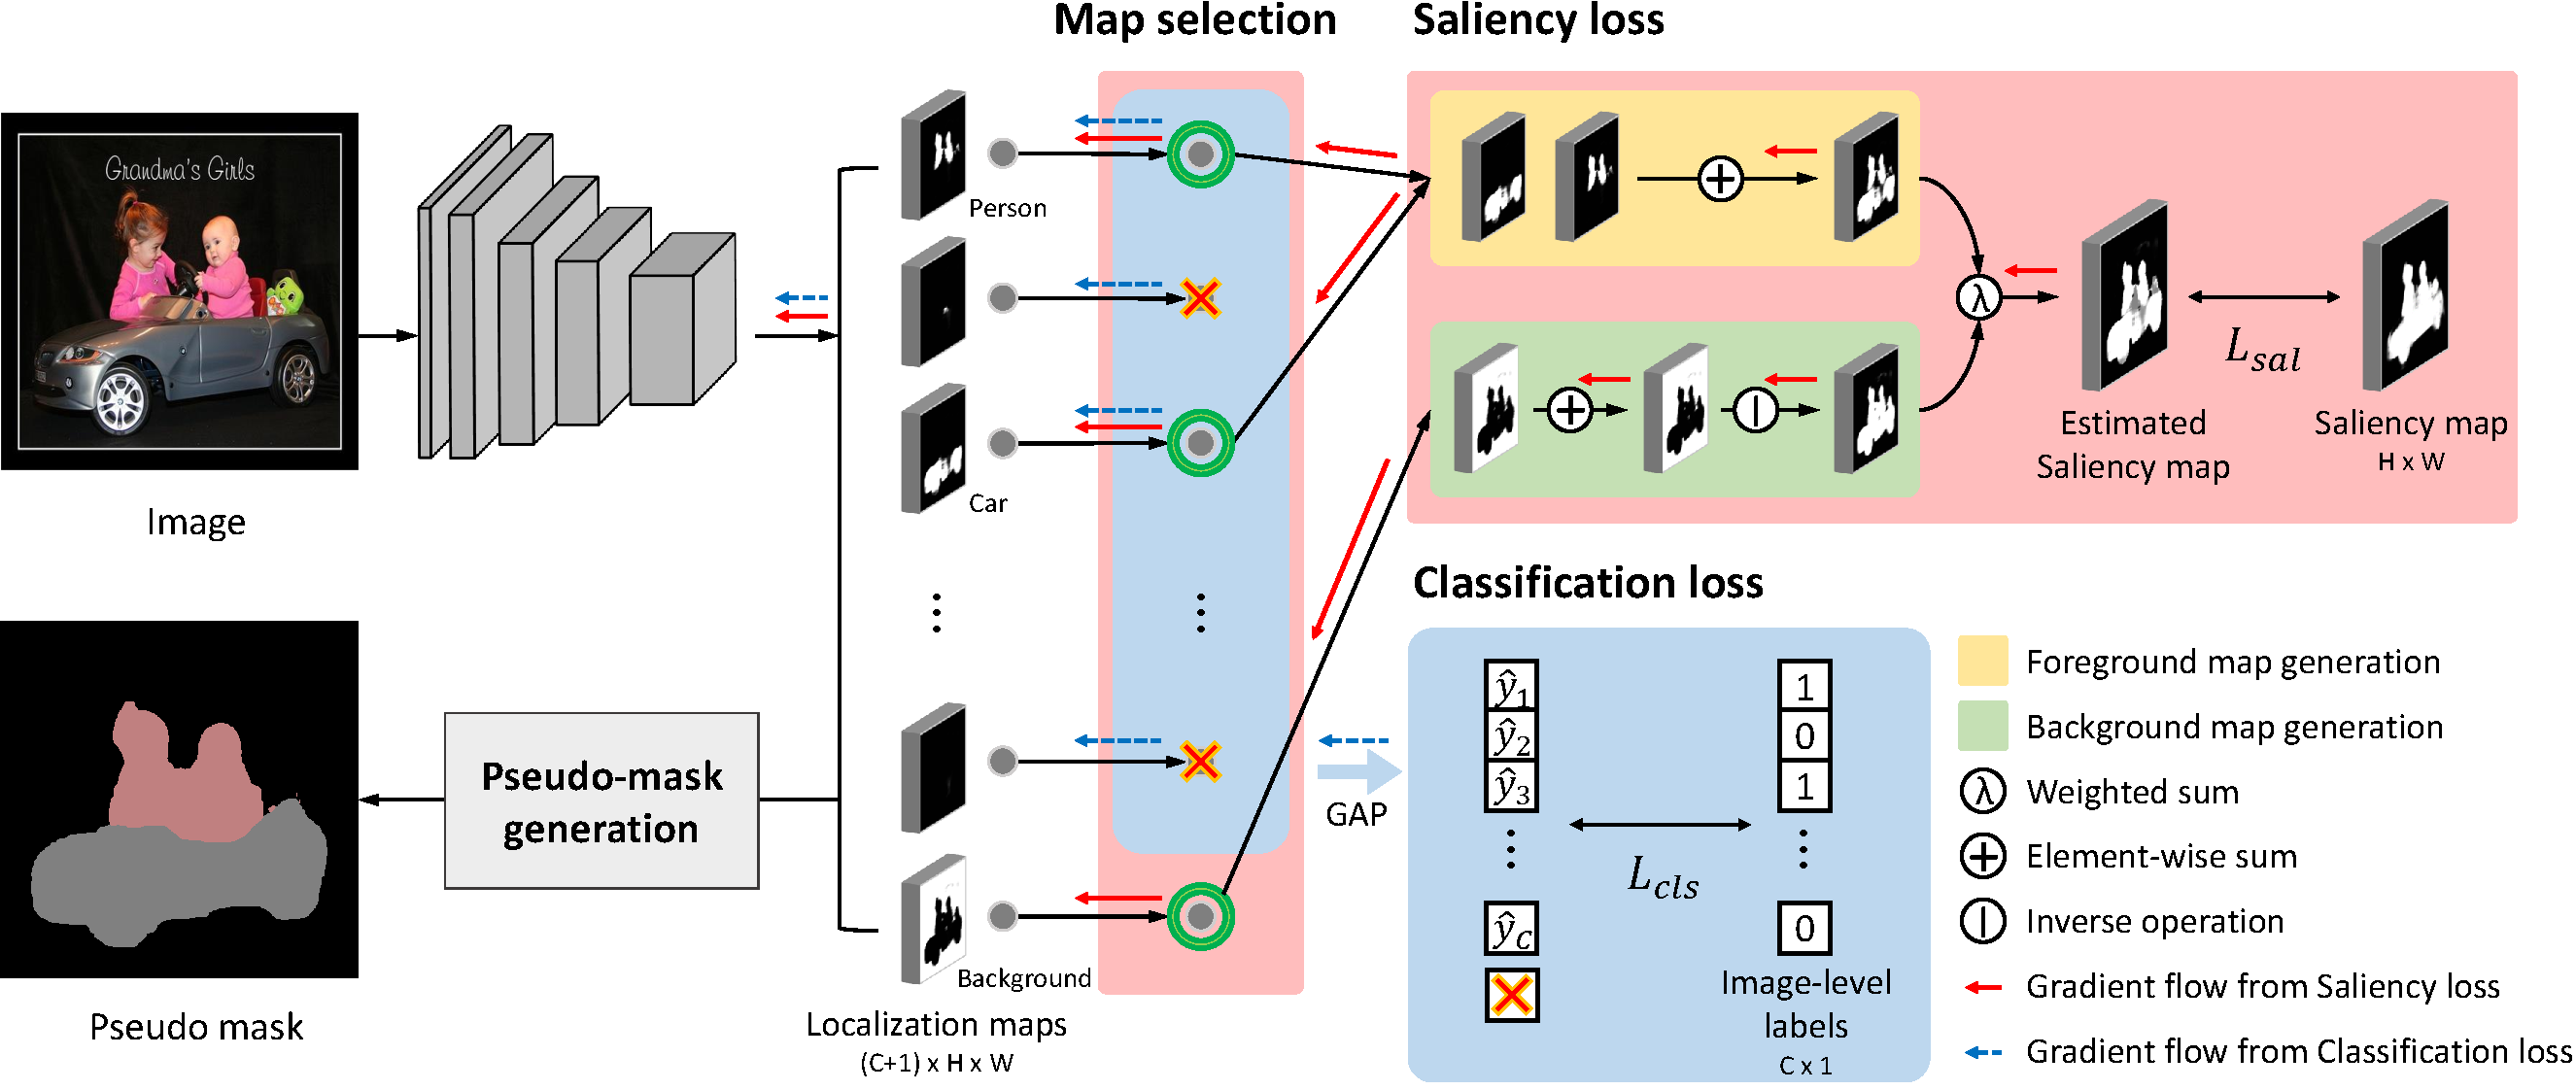
\includegraphics[width=16cm]{figures/framework.pdf}
\caption{我々のEPSの全体的なフレームワーク。$C+1$のローカライゼーションマップがバックボーンネットワークから生成されます。実際の顕著性マップは、既製の顕著性検出モデルから生成されます。ターゲットラベルのためのいくつかのローカライゼーションマップは、推定顕著性マップを生成するために選択的に使用されます(セクション~\ref{section3.2})。全体的なフレームワークは、顕著性損失と分類損失と共に共同で訓練されます(セクション~\ref{section3.3})。} \vspace{-2mm}
\label{fig:framework}
\end{figure*}
